\documentclass{report}

\usepackage{titlesec}
\usepackage[nottoc, numbib]{tocbibind}  % Automatically adds Bibliography to TOC
\usepackage[toc,page]{appendix}  % For appendix formatting
\usepackage{pdfpages}
\usepackage{hyperref}      % Voor hyperlinks
\usepackage[dutch]{babel}  % Gebruik de Nederlandse taal
\usepackage{todonotes}
\usepackage[utf8]{inputenc}
\usepackage{graphicx}
\usepackage{amsmath}
\usepackage{listings}
\usepackage{geometry}
\usepackage{xcolor}


\begin{document}

    % Titelpagina
    \begin{titlepage}
        \centering
        % \centering
        % Title of the document
        \vspace*{2cm}  % Adjusts vertical space from the top of the page
        \Huge
        \textbf{Beroepsproduct DDDQ: Casus top 2000} \\[1.5cm]  % Add your document's title here

        % Author name(s)
        \large
        \textbf{Auteurs} \\[0.25cm]
        \textnormal{Geo Bouwmeestern, Neo Hop \& Julian van Zwol} \\[2.25cm]

        % Additional information (e.g., institution, course name)
        \textit{HAN University of applied sciences} \\[0.25cm]
        \textit{Academie IT en Mediadesign} \\[0.25cm]
        \textit{I-ADB 2024/2025 - Advanced Databases (deeltijd)} \\[0.25cm]

        % Date
        \vfill
        \today \\[0.25cm]  % Use \today for today's date or specify a custom date like '1 January 2025'
        \textbf{Versie 1.0} \\[1cm]
    \end{titlepage}

    \renewcommand{\contentsname}{Inhoud}
    \tableofcontents

    \chapter{Inleiding}\label{chapter:Inleiding}

    \chapter{Onderzoek Datakwaliteit}\label{chapter:Onderzoek Datakwaliteit}

        \section{Duiding Databasestructuur}

            \subsection{Database Diagram}

                \begin{figure}
                    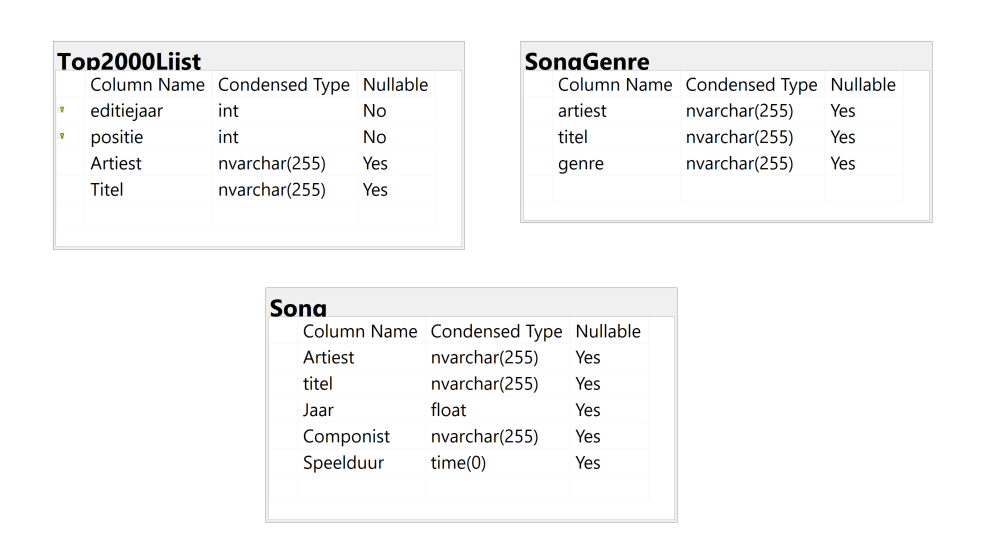
\includegraphics[width=\linewidth]{databasestructuur.png}
                    \caption{Generated diagram from SSMS.}
                    \label{fig:boat1}
                \end{figure}

            \subsection{Toelichting}

                \todo{Invulling geven.}

        \section{Controle op Schending Primary key}
            Voor de controle op schending van de (logische) primary keys is gebruikt gemaakt van een query 
            die records binnen de betreffende tabel groepeert op de (logische) primary key 
            en vervolgens controleert of hier duplicaten tussen zitten.

            \subsection{Check op tabel Top2000Lijst}
                Uitvoering van de SQL select query in bijlage ~\ref{section:checks_pk} 
                resulteerde in geen schending van de primary key.

            \subsection{Check op tabel SongGenre}
                Uitvoering van de SQL select query in bijlage ~\ref{section:checks_pk} 
                resulteerde in geen schending van de logische primary key.

            \subsection{Check op tabel Song}
                Uitvoering van de SQL select query in bijlage ~\ref{section:checks_pk} 
                resulteerde in geen schending van de logische primary key.

        \section{Controle op schending van Referentiële integriteit}

            \subsection{Check on Top2000Lijst's (logically) referentie naar Song}
                Uitvoering van de SQL select query in bijlage ~\ref{section:checks_ref_int} 
                resulteerde in schending van de referentiële integriteit op \textbf{122} records.

            \subsection{Check on SongGenre's (logically) referentie naar Song}
                Uitvoering van de SQL select query in bijlage ~\ref{section:checks_ref_int} 
                resulteerde in schending van de referentiële integriteit op \textbf{7} records.

        \section{Controle op Derde Normaalvorm (3NF)}

            Volgens de theorie is een tabel in Eerste Normaalvorm (1NF) als elke cel een atomaire waarde bevat. 
            Elke cel voor alle kolommen voor elke tabel bevat een redelijke atomaire (= ondeelbare) waarde, 
            behalve de kolom 'Componist' in tabel 'Song'. 
            Deze bevat een door komma's gescheiden lijst met waarden die de Eerste Normaalvorm schendt. 
            Dit betekent dat de tabel niet genormaliseerd is en zeker niet in Derde Normaalvorm.

        \section{Controle op Integriteitregels}

            \paragraph{IR1. Een song staat maximaal één keer in een editie van de Top 2000.}
                Uitvoering van de SQL select query in bijlage ~\ref{section:checks_int_rules} 
                resulteerde in schending van de Integriteitregel op \textbf{2} records.

            \paragraph{IR2. Elke song die in een editie van de Top 2000 staat, 
            is vóór of ìn het jaar van de betreffende editie uitgebracht.}
                Uitvoering van de SQL select query in bijlage ~\ref{section:checks_int_rules} 
                resulteerde in geen schending van de Integriteitregel.

            \todo{Zijn er nog andere integriteitregels? Wordt expliciet naar verwezen in rubriek.}

        \section{Controle op Datakwaliteitsdimensie \textit{Completeness}}

            Uitvoering van de SQL select query in bijlage ~\ref{section:checks_com} 
            resulteerde in een percentage van \textit{96.00\%} 
            van nummers in de Top2000 lijst van 2019 waarvan voor elk gegeven attribuut een waarde beschikbaar is.

            Uitvoering van de SQL select query in bijlage ~\ref{section:checks_com} 
            resulteerde in een percentage van \textit{96.00\%} 
            van nummers in de Top2000 lijst van 2019 waarvan voor elk gegeven attribuut een waarde beschikbaar is.

            \todo{Zijn er nog meer referentiele integriteit regels?}

        \section{Controle op Datakwaliteitsdimensie \textit{Accuracy}}

            \todo{Invulling geven.}
            \todo{Zijn er typefouten?}
            \todo{Zijn er standaard waardes zoals: 1-1-1900}

            \subsection{Geen uniforme schrijfwijze}
                Uitvoering van de SQL select query in bijlage ~\ref{section:checks_acc} 
                resulteerde in \textbf{226} "unieke" records.
                Echter hebben sommige genres verschillende schrijfwijzes en daarmee dus geen uniforme manier om genres weer te geven.
                Enkele voorbeelden staan hieronder:

                \begin{table}[h!]
                    \centering
                    \begin{tabular}{|l|l|l|}
                    \hline
                    \textbf{Optie 1} & \textbf{Optie 2} & \textbf{Optie 3} \\ \hline
                    alternatieve rock & alternatieve rock & - \\ \hline
                    elektronisch & elektronische muziek & elektroniche muziek \\ \hline
                    hard rock & hardrock & - \\ \hline
                    Keltisch & Keltische muziek & - \\ \hline
                    kerstlied & kerstmuziek & - \\ \hline
                    klassiek & klassieke muziek & - \\ \hline
                    poppunk & popunk & - \\ \hline
                    psychedelic rock & psychedelische rock & - \\ \hline
                    rock-'n -roll & rock-'n-roll & - \\ \hline
                    trash metal & trashmetal & - \\ \hline
                    \end{tabular}
                    \caption{Alternatieve schrijfwijzes}
                \end{table}
                
            \todo{uniforme manier?}

        \section{Verbeteringen m.b.t. Data Intension}

            \todo{Invulling geven.}

        \section{Verbeteringen m.b.t. Data Extension}

            \todo{Invulling geven.}

        \section{Overige constateringen}

            \begin{itemize}
                \item The attribute 'artiest' regards a person and should therefore be it's own entity (table).
                \item The table 'SongGenre' is not normalized past the First Normal Form and has therefore a lot of redundant data.
                \item Three
            \end{itemize}

    \renewcommand{\listfigurename}{Lijst van figuren}
    \addcontentsline{toc}{chapter}{\listfigurename}
    \listoffigures

    \chapter{Bijlage}\label{chapter:Bijlage}
    
    \appendix  % Marks the start of the appendix section

    \lstset{
        keywordstyle=\color{blue},       % Keywords in blue
        stringstyle=\color{red},         % Strings in red
        commentstyle=\color{green!80!black},      % Comments in green
        numbers=left,                    % Show line numbers on the left
        language=SQL,                    % Syntax highlighting for SQL
        basicstyle=\ttfamily,            % Monospaced font
        frame=single,                    % Frame around the code
        breaklines=true,                 % Automatic line breaking
        inputencoding=utf8,              % UTF-8 encoding for the input file
    }

    \section{Controle op Schending Primary key}\label{section:checks_pk}

    \lstinputlisting[language=SQL]{checks_pk.sql}

    \section{Controle op Schending van Referentiële integriteit}\label{section:checks_ref_int}

    \lstinputlisting[language=SQL]{checks_ref_int.sql}

    \section{Controle op Integriteitregels}\label{section:checks_int_rules}

    \lstinputlisting[language=SQL]{checks_int_rules.sql}

    \section{Controle op Datakwaliteitsdimensie \textit{Completeness}}\label{section:checks_com}

    \lstinputlisting[language=SQL]{checks_com.sql}

    \section{Controle op Datakwaliteitsdimensie \textit{Accuracy}}\label{section:checks_acc}

    \lstinputlisting[language=SQL]{checks_acc.sql}

\end{document} % This is the end of the document